\section{Introduction}
\subsection{Design Problem}
The goal of this project is to design an SCOMP wall following program
that enables the Amigobot to follow walls. The design solution meets
the following specications:

\begin{enumerate}
\item Use an eight bit velocity command where \(+127\) (\verb+0x007F+)
  is full speed forward, \(-127\) (\verb+0xFF81+) is full speed
  reverse, and zero is stop.
\item Control position by reading the cumulative rotation counter of
  the wheel.
\item Use velocity feedback and position feedback from the wheels via
  the existing optical encoder peripheral.
\item Provide a start button to begin execution after the robot is
  placed adjacent to a wall.
\item Use existing sonar and velocity control peripherals to issue
  commands to each wheel.
\item Travel parallel to a wall at a distance of 20 cm.
\item Select by switch or recompile to follow left or right walls.
\end{enumerate}

The Amigobot was expected to navigate a course without collisions and
in a specified time frame. A sample course layout is shown in
Fig.~\ref{samplecourse}.

In addition to the required specifications, the wall following program
improved the user interface of the robot by enhancing the 7-segment,
LCD, and LED displays.

\begin{figure}[h!]
  \centering \cprotect \fbox{
    \begin{minipage}{3.5in}
      \centering
      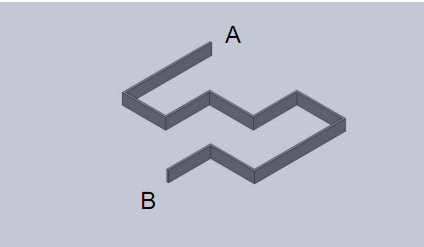
\includegraphics[width =
      \textwidth]{./graphics/course.png}
      \cprotect \caption{Sample course layout for robotic
        wall-following.}
      \label{samplecourse}
    \end{minipage}
  }\end{figure}

\subsection{Design Solution}

The SCOMP program written for the design problem is a state machine
consisting of four states. In the ``forward'' state, the
robot follows a straight trajectory until it senses a wall in front or
no wall is sensed. If the Amigobot senses a wall in front of it, the program
switches to the ``inside turn'' state, turns \(90^\circ\), then proceeds
on a straight trajectory. If no wall is sensed, the Amigobot adjusts
inward until it is parallel to the wall. The two adjustment states,
``adjust outward'' and ``adjust inward,'' maintain parallel motion to the
wall by correcting the robot trajectory when the measured distance to
the wall is not within an acceptable range of \(20\pm 1\) cm.

A switch is used to toggle between following a wall on the left side
or on the right side of the robot. The switch position activates the
ultrasonic sensors on one side of the robot and determines clockwise
or counterclockwise turning direction.

The initial approach discussed in the proposal (see
Appendix~\ref{proposal}) implemented an
additional ``outside turn'' state. During testing, it was discovered
that the state causes the robot to turn prematurely and collide with
the wall whenever the robot was not parallel to the wall. To overcome
this challenge, the team used the ``adjust inward'' state to make
incremental turns around an outside wall corner.

Additionally, the initial design called for one sensor reading from
the lateral region of the robot and one from the forward region of the
robot. During
testing it was discovered that accuracy in maintaining the set
distance improved when the minimum value of two sensors in the lateral
and forward regions were used as inputs to the states.

The role of the LCD display had to be altered when the team ran into
issues of consistency. The LCD display was initially expected to show
the moving state the robot is in. Due to the display not working
consistently, it was changed to show the basic startup states.

The design demonstration met most of the specifications outlined
above. The robot successfully completed the course for both the left
and right sided walls. It received an accuracy bonus for maintaining
the desired 20 cm distance when following the right wall. However, it
was unable to earn the accuracy bonus when following the left wall.
